% =====================================================================
%  Comunicação Oral · XII Bienal da SBM · UFRN, Natal-RN · agosto 2026
%  Autor: Pablo Nogueira Grossi (G6 LLC)
%  Tema: T2 — ajustar na submissão conforme eixo temático
%  Título: O Princípio do Cajueiro — Inglês para Pesquisadores Matemáticos
%          via TOGT (uma aplicação do GUT pedagógico)
% =====================================================================
\documentclass[11pt,a4paper]{article}

\usepackage[utf8]{inputenc}
\usepackage[T1]{fontenc}
\usepackage{lmodern}
\usepackage[a4paper,margin=2cm,top=2.8cm,bottom=2.2cm,headheight=18mm,headsep=6mm]{geometry}
\usepackage{amsmath,amssymb,amsthm}
\usepackage{booktabs}
\usepackage{enumitem}
\usepackage{graphicx}
\usepackage{fancyhdr}
\usepackage[hidelinks]{hyperref}
\renewcommand{\tablename}{Tabela}
\renewcommand{\figurename}{Figura}

% ─── Cabeçalho e rodapé institucionais (UFRN + XII Bienal SBM 2026) ──
\newcommand{\institutionalheader}{%
  \fancyhf{}%
  \fancyhead[L]{\raisebox{-0.35\height}{
\includegraphics[height=9mm]{assets/ufrn-logo.png}}}%
  \fancyhead[R]{\raisebox{-0.35\height}{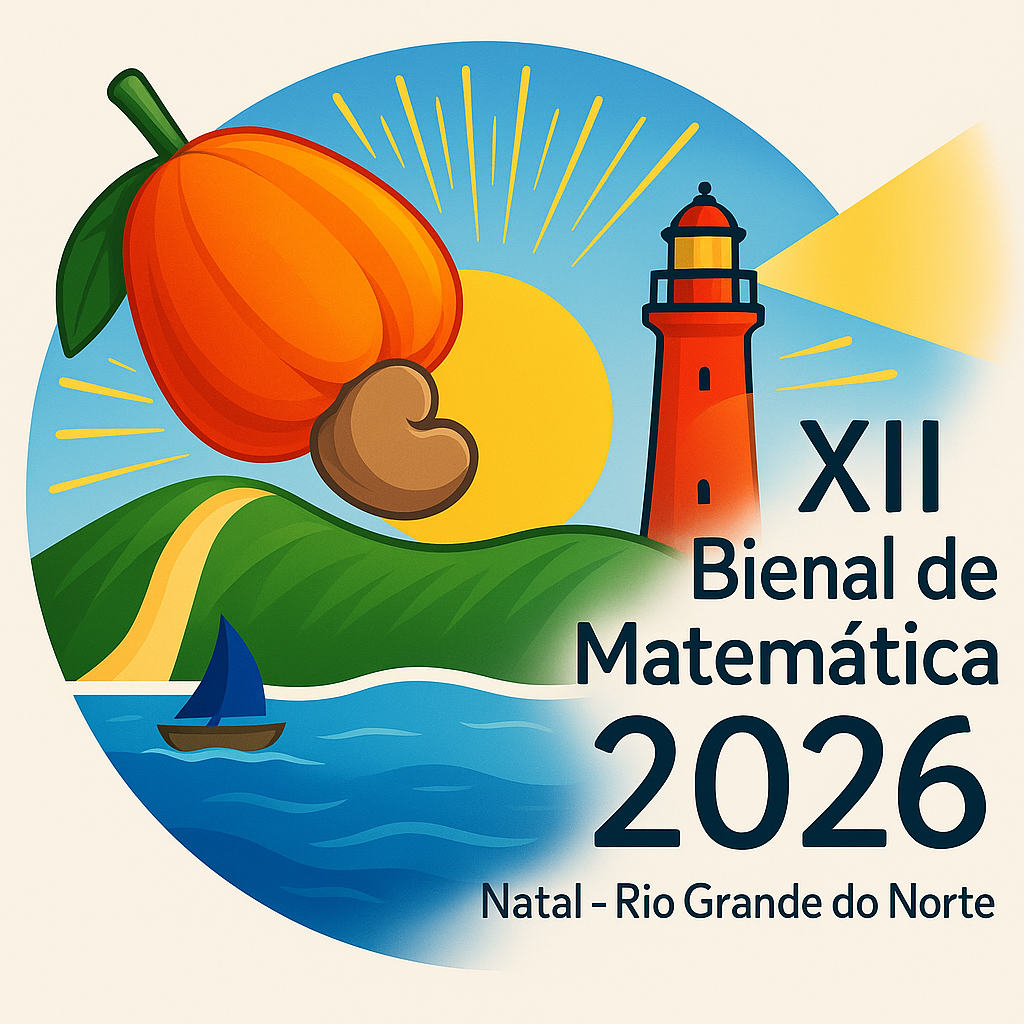
\includegraphics[height=13mm]{assets/bienal-2026-logo.png}}}%
  \fancyfoot[L]{\tiny\textcopyright\ 2026 Pablo N. Grossi / G6 LLC \textbullet\ CC BY 4.0 \textbullet\ XII Bienal da SBM 2026}%
  \fancyfoot[R]{\tiny \thepage}%
  \renewcommand{\headrulewidth}{0.3pt}%
  \renewcommand{\footrulewidth}{0.3pt}%
}
\pagestyle{fancy}\institutionalheader
\fancypagestyle{plain}{\institutionalheader}

\title{\textbf{O Princípio do Cajueiro}\\[0.3em]
\large Inglês para Pesquisadores Matemáticos via TOGT ---\\
uma aplicação do \emph{Grand Unified Theory} pedagógico}
\author{Pablo Nogueira Grossi\\
\small G6 LLC\\
\small \texttt{brodananda@gmail.com}}
\date{Submissão à XII Bienal da SBM --- UFRN, Natal-RN --- 2026}

\setlength{\parskip}{0.4em}
\setlength{\parindent}{0pt}

\begin{document}

\maketitle

% =====================================================================
\section*{Modalidade e Duração}
\noindent
\textbf{Modalidade:} Comunicação Oral (palestra curta).\quad
\textbf{Duração:} 45 minutos --- 40 minutos de exposição + 5 minutos para perguntas.\quad
\textbf{Público-alvo:} pesquisadores em Matemática, pós-graduandos e professores universitários brasileiros que precisam publicar, apresentar e arbitrar trabalhos em língua inglesa.

% =====================================================================
\section*{Resumo}

O cajueiro de Pirangi, a 20~km do campus da UFRN, estende-se por mais de 8.500~m$^2$: um tronco central cujos ramos, ao tocarem o solo, enraízam-se e se tornam tronco --- um organismo que cresce por propagação lateral preservando a identidade do sistema inicial. Esta comunicação propõe que a aquisição de inglês acadêmico por pesquisadores brasileiros em matemática segue, estruturalmente, o mesmo princípio. Chamamos este padrão de \emph{Princípio do Cajueiro}.

Três observações o motivam. (i)~\emph{Empírica:} pesquisadores brasileiros têm inglês \emph{funcional} para leitura, mas déficit de \emph{produção} (escrita de \emph{papers}, \emph{talks}, \emph{referee reports}). (ii)~\emph{Teórica:} o inglês acadêmico tem um tronco comum (500 palavras-raiz, tempos verbais matemáticos, sete movimentos retóricos CARS de Swales) e raízes laterais por subárea. (iii)~\emph{Estrutural:} a aquisição segue a correspondência CEFR $\to$ TOGT~[1]: cada nível é uma camada estrutural-cognitiva; a aquisição \emph{não é linear} mas \emph{propagativa} --- um nível se estabelece quando o anterior se solidifica o bastante para gerar novo ponto de contato com o solo.

A apresentação aplica o \emph{Grand Unified Theory} pedagógico~[2], que unifica aquisição CEFR, progressão TOGT e dinâmica contínua via operadores de contração, curvatura, filtro e desdobramento, ao caso específico da produção acadêmica em inglês por pesquisadores brasileiros.

% =====================================================================
\section*{As Quatro Estruturas do Cajueiro}

A metáfora botânica é mais do que ornamental: cada parte do cajueiro corresponde a uma camada pedagógica com regras próprias.

\begin{enumerate}[leftmargin=2em,itemsep=0.15em]
  \item \textbf{Raiz Profunda.} Tronco de \emph{core academic English}: 500 palavras-raiz, tempos verbais matemáticos (presente para teoremas, pretérito para resultados publicados), e os 7 movimentos CARS de Swales. Sem o tronco, nada cresce.
  \item \textbf{Raízes Laterais.} Extensões por subárea: o inglês de um geômetra diferencial (``\emph{smooth}'', ``\emph{fiber}'', ``\emph{this manifold admits}'') difere do de um combinatorialista (``\emph{sharp}'', ``\emph{there is a bijection}''). Só se formam \emph{após} o tronco.
  \item \textbf{Copa.} Output de alto custo: \emph{talks}, \emph{grant proposals}, \emph{referee reports}. Pequena mas concentra toda a função comunicativa. A maioria dos cursos falha por começar pela copa.
  \item \textbf{Propagação.} A primeira apresentação em ambiente protegido (grupo de pesquisa, seminário interno) estende o tronco. Assistida por \emph{scaffold} de prompts LLM~[1], adaptado às 14 semanas de um programa CEFR $\to$ TOGT completo.
\end{enumerate}

% =====================================================================
\section*{Estrutura da Apresentação (40 minutos)}

\begin{table}[h]
\centering
\small
\begin{tabular}{@{}lp{0.68\linewidth}@{}}
\toprule
\textbf{Tempo} & \textbf{Conteúdo} \\
\midrule
0--5 min   & Motivação. O paradoxo brasileiro: alta competência em leitura, baixa produção escrita e oral. Dados de uma pesquisa informal com pós-graduandos do IMPA (2025--2026). \\
5--12 min  & O \emph{Grand Unified Theory} pedagógico. Correspondência CEFR $\to$ TOGT (Tabela~\ref{tab:cefr}). Por que um nível estrutural funciona como ponto de apoio para o próximo. \\
12--22 min & O Princípio do Cajueiro em detalhe: as quatro estruturas (raiz profunda, laterais, copa, propagação). Contraexemplos: por que os cursos que começam pela copa (``\emph{business English for scientists}'') falham de forma previsível. \\
22--32 min & O programa de 14 semanas. Cronograma semana-a-semana mostrando qual estrutura é desenvolvida em cada bloco, qual LLM-prompt corresponde a qual exercício, e quais predições falsificáveis o GUT faz sobre a curva de aquisição. \\
32--38 min & Implementação em laboratórios de pesquisa: como adaptar o programa a um grupo de 4--8 pós-graduandos; que tipo de facilitador é necessário (alguém com C1+, não precisa ser nativo); como medir progresso sem depender de exames externos. \\
38--40 min & Conclusão. O cajueiro é um organismo, não um currículo: abre discussão. \\
\bottomrule
\end{tabular}
\caption{Cronograma da Comunicação Oral.}
\end{table}

% =====================================================================
\section*{Correspondência CEFR $\to$ TOGT --- tabela de apoio}

\begin{table}[h]
\centering
\small
\begin{tabular}{@{}cccl@{}}
\toprule
CEFR & TOGT & Operador & Marco produtivo em matemática \\
\midrule
A1 & L$_0$ & C (contração) & Lê \emph{abstract}. \\
A2 & L$_1$ & C $\to$ K & Resume em 3 frases um artigo da sua subárea. \\
B1 & L$_2$ & K (curvatura) & Apresenta 10 min em seminário interno em inglês. \\
B2 & L$_3$ & K $\to$ F & Escreve primeiro rascunho de \emph{introduction}. \\
C1 & L$_4$ & F (filtro) & Submete \emph{referee report} em inglês. \\
C2 & L$_5$ & F $\to$ U & Defende \emph{grant proposal} em arguição internacional. \\
Nativo-like & L$_6$ & U (desdobramento) & Escreve com voz autoral; escolhe registro por efeito. \\
\bottomrule
\end{tabular}
\caption{Correspondência CEFR $\to$ TOGT e marcos matemáticos. Adaptado de~[1], Capítulo 6.\label{tab:cefr}}
\end{table}

% =====================================================================
\section*{Contribuição e Predições Falsificáveis}

A comunicação apresenta três contribuições distintas:

\begin{enumerate}[leftmargin=2em,itemsep=0.2em]
  \item \textbf{Metodológica.} Um currículo de 14 semanas com materiais prontos (prompts, folhas de trabalho, critérios de avaliação) para grupos de pesquisa brasileiros implementarem internamente, sem custo adicional, com resultados mensuráveis em 4 meses.
  \item \textbf{Teórica.} O \emph{mapping} explícito entre os níveis CEFR e os níveis TOGT, testável por observação longitudinal: \emph{prevê-se} que a transição B1 $\to$ B2 coincide com a transição operador $K \to F$ no sentido GTCT, isto é, com a emergência da capacidade produtiva de \emph{filtrar} linguagem técnica para linguagem de divulgação.
  \item \textbf{Local.} A ancoragem simbólica no cajueiro de Pirangi como \emph{topos} norte-rio-grandense oferece ao programa uma identidade regional --- relevante para pesquisadores brasileiros que frequentemente se sentem deslocados ao adotar modelos pedagógicos estrangeiros.
\end{enumerate}

\noindent \textbf{Predição falsificável principal:} se o Princípio do Cajueiro é correto, então um programa de 14 semanas com foco no tronco (semanas 1--7) antes das raízes laterais (semanas 8--14) produzirá \emph{ganho maior} em produção escrita (medido por \emph{words-per-draft}, qualidade de \emph{abstract}) do que um programa de mesma duração com a ordem invertida. O estudo-piloto está planejado para 2026--2027.

% =====================================================================
\section*{Bibliografia}

\begin{enumerate}[leftmargin=2em,itemsep=0em,label={[\arabic*]}]
  \item GROSSI, P.~N. Helical Attractors on Contact 3-Manifolds. In: \emph{Principia Orthogona}, Vol.~IV. G6 LLC, 2026. \url{https://totogt.github.io/3M/}.
  \item GROSSI, P.~N. \emph{Generative Temporal Contact Theory (GTCT) --- Axioms, Operators, and the Operator Chain}. Manuscript, 2026. \url{https://github.com/TOTOGT/GTCT}.
  \item SWALES, J.~M. \emph{Genre Analysis: English in Academic and Research Settings}. Cambridge: CUP, 1990.
  \item COUNCIL OF EUROPE. \emph{Common European Framework of Reference for Languages: Learning, Teaching, Assessment --- Companion Volume}. Strasbourg, 2020.
  \item HYLAND, K. \emph{Disciplinary Discourses: Social Interactions in Academic Writing}. Harlow: Longman, 2000.
\end{enumerate}

\vspace{1em}
\noindent\rule{\linewidth}{0.3pt}\\[0.3em]
\footnotesize
\emph{Submissão à XII Bienal da Sociedade Brasileira de Matemática. UFRN, Natal-RN, 3--7 de agosto de 2026. Categoria: Comunicação Oral (40~min + 5~min Q\&A). Código de tema: T2 (a confirmar no portal conforme eixo temático selecionado --- naturalmente se enquadra em \emph{Ensino e Popularização da Matemática} ou \emph{Formação de Pesquisadores}).}

\end{document}
